\begin{figure}[!htbp]\centering
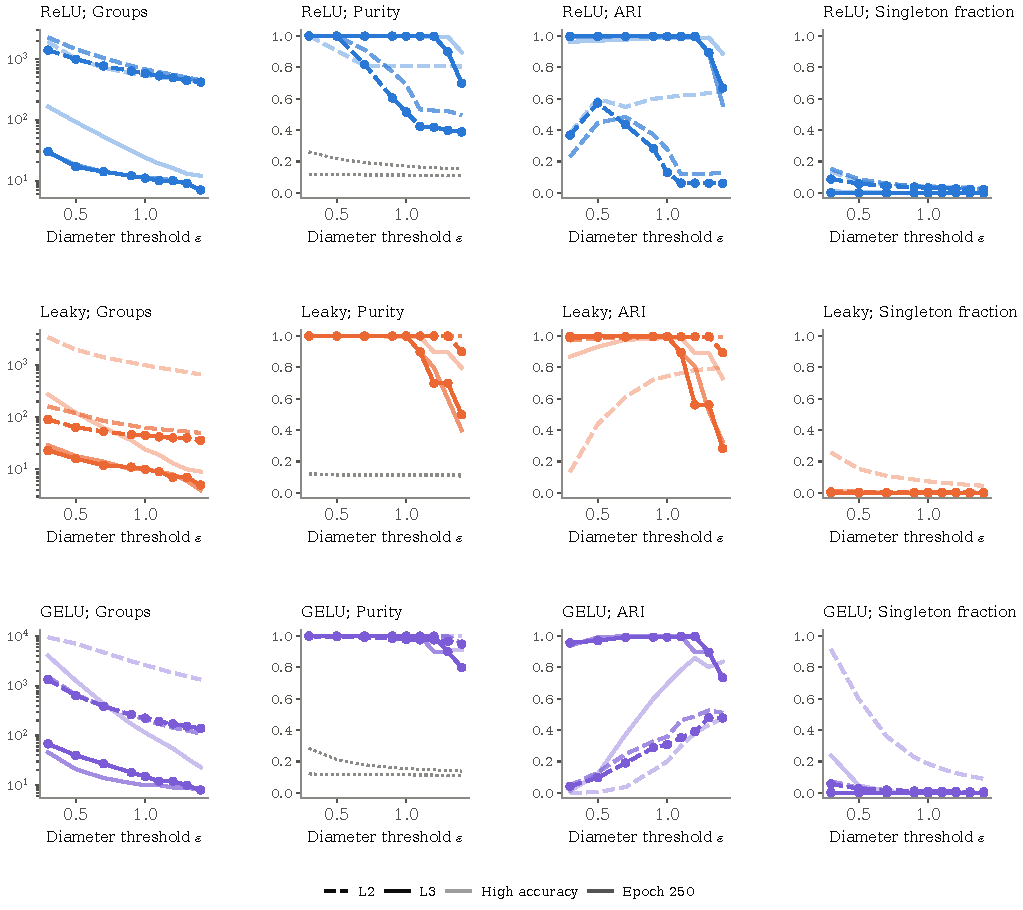
\includegraphics[width=6.138in]{cluster_diameters.pdf}
\caption{Diameter-controlled clustering in the same width-128 networks, seed 0. Rows compare activations; columns show group count, label purity, adjusted Rand index and the fraction of samples in singleton groups. Solid and dashed curves denote L3 and L2. Opacity increases from high accuracy to epoch 250 and epoch 500; endpoint curves have markers. Dotted purity controls shuffle labels at fixed group sizes. L3 forms class-aligned groups for every activation, whereas L2 behavior depends on activation. High purity carried by singletons is distinguished from grouping whole classes.}\label{fig:cluster-diameters}
\end{figure}
\FloatBarrier
